
% This LaTeX was auto-generated from MATLAB code.
% To make changes, update the MATLAB code and republish this document.

\documentclass{article}
\usepackage{graphicx}
\usepackage{color}

\sloppy
\definecolor{lightgray}{gray}{0.5}
\setlength{\parindent}{0pt}

\begin{document}

    
    
\section*{Lab 5}

\begin{par}
The following lab explores the convergence of Chebyshev interpolation at Chebyshev extreme points for oscillating function based on their rate of oscillation. I will also discuss the order of convergence for the Chebyshev coefficients for these interpolating polynomials.
\end{par} \vspace{1em}

\subsection*{Contents}

\begin{itemize}
\setlength{\itemsep}{-1ex}
   \item f(x)
   \item g(x)
   \item h(x)
\end{itemize}
\begin{par}
The following code calculates the Chebyshev coefficients for interpolating f(x), g(x), and h(x) at the Chebyshev extreme points with omega ranging from 10 to 100. f, g, and h are shown below.
\end{par} \vspace{1em}
\begin{par}
$f(x) = sin(\omega x + 1)$
\end{par} \vspace{1em}
\begin{par}
$g(x) = \frac{sin(\omega x + 1)}{4 (x - 0.1^2) + 1}$
\end{par} \vspace{1em}
\begin{par}
$h(x) = sin(\omega x + 1) | (x - 0.1^3)|$
\end{par} \vspace{1em}
\begin{par}
The Discrete Cosine Transform is used to calculate these Chebyshev coefficients. The code for that is shown below.
\end{par} \vspace{1em}
\begin{verbatim}
disp(fileread("dct1.m"));
\end{verbatim}

        \color{lightgray} \begin{verbatim}%=======================================
% DCT-1 : Discrete cosine transform
%---------------------------------------
% Code adapted from
% P. Moin, Fundamentals of Engineering Numerical Analysis (2010)
%
% Computes the same result as exemplified in Chebseries.m
% but uses the built-in Fast Fourier Transform fft()
%
% The following are equivalent:
%    c = DCT1(exp(cos((0:16)./16.*pi))')
%    c = Chebseries(@(x) exp(x), 16)
%
%=======================================
function y=dct1(f_vals)

N      =length(f_vals);
y      =[f_vals;flipud(f_vals(2:N-1,:))];
y_ft   =fft(y);
y      =real(y_ft(1:N,:)/(N-1));
y(1,:) = y(1,:)/2;
y(N,:) = y(N,:)/2;

\end{verbatim} \color{black}
    \begin{verbatim}
close all;

n = 10000;
j = 0:n;
x = cos((0:n) .* pi ./ n);

omega = linspace(10, 100, 10);
c_f = zeros(n+1, 10);
c_g = zeros(n+1, 10);
c_h = zeros(n+1, 10);
for k = 1:10
    f = sin(omega(k) .* x + 1);
    g = (sin(omega(k) .* x + 1)) ./ (4 .* (x - 0.1) .^ 2 + 1);
    h = (sin(omega(k) .* x + 1)) .* abs((x - 0.1) .^ 3);

    c_f(:, k) = abs(dct1(f'));
    c_g(:, k) = abs(dct1(g'));
    c_h(:, k) = abs(dct1(h'));
end
\end{verbatim}


\subsection*{f(x)}

\begin{par}
The graph below plots the Chebyshev coefficients c\_k against k in a semilogy scale. From the plots, it is clear that there are three main phases: the convergence phase with the pre-convergence phase before it and the round-off phase afterwards. For omega=20, the convergence phase ranges from k=20 to k=50. For omega=60, the convergence phase ranges from k=60 to k=110. For omega=100, the convergence phase ranges from k=100 to k=150.
\end{par} \vspace{1em}
\begin{verbatim}
kstart = 10;
kend = 180;
k = linspace(kstart, kend, kend-kstart+1);
figure1 = figure();
semilogy(k, c_f(k, 2), '-r', k, c_f(k, 6), '-b', k, c_f(k, 10), '-g');
xlabel('k');
ylabel('|c_k|');
title('Convergence Phases for f(x)');
legend('\omega = 20', '\omega = 60', '\omega = 100');
\end{verbatim}

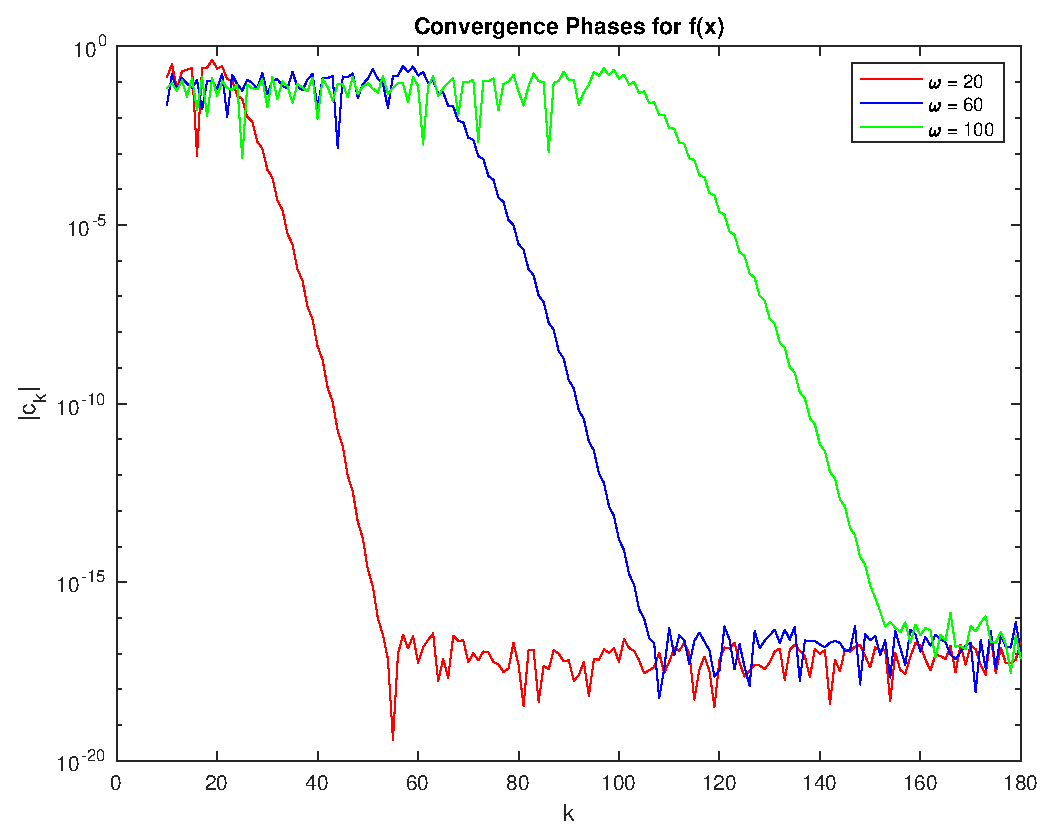
\includegraphics [width=4in]{Lab5_01.eps}
\begin{par}
Since f(x) has an infinite radius of convergence and is analytic in a Bernstein ellipse of an arbitrarily large rho, the Chebyshev coefficients can be bounded by O(rho\^{}-k). Hence, c\_k can be bounded by M * rho\^{}-k. Since rho can be arbitrarily large, the best combination of rho and M that I found are 3 and 10000000000, which is shown below in the graph.
\end{par} \vspace{1em}
\begin{verbatim}
rho = 3;
M = 10000000000;
kstart = 10;
kend = 150;
k = linspace(kstart, kend, kend-kstart+1);
figure7 = figure();
semilogy(k, c_f(k, 2), (20:55), M ./ (rho .^ (20:55)), 'LineWidth', 2);
xlabel('k');
ylabel('|c_k|');
title('Chebyshev Coefficient Bound (\rho =3 and M=10000000000)');
legend('\omega = 20', 'M \rho ^{-k} ');
\end{verbatim}

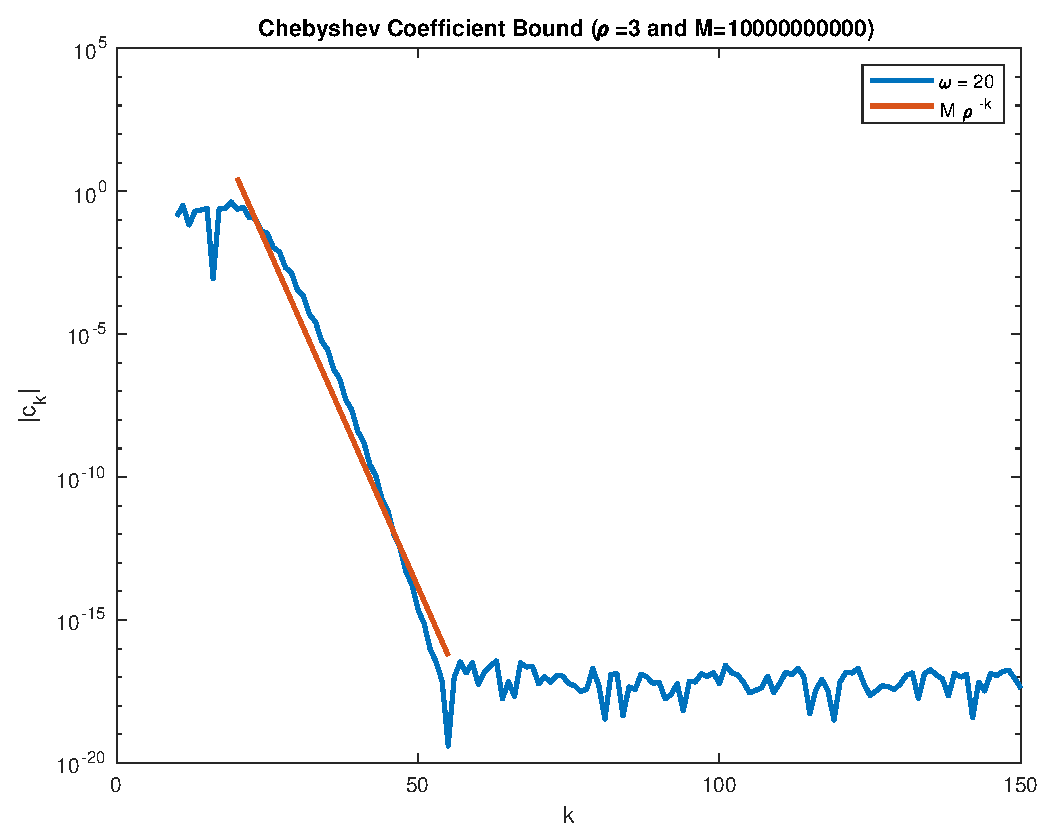
\includegraphics [width=4in]{Lab5_02.eps}


\subsection*{g(x)}

\begin{par}
The graph below plots the Chebyshev coefficients c\_k against k in a semilogy scale. For omega=20, the convergence phase ranges from k=20 to k=100. For omega=60, the convergence phase ranges from k=60 to k=150. For omega=100, the convergence phase ranges from k=100 to k=180.
\end{par} \vspace{1em}
\begin{verbatim}
kstart = 10;
kend = 220;
k = linspace(kstart, kend, kend-kstart+1);
figure2 = figure();
semilogy(k, c_g(k, 2), '-r', k, c_g(k, 6), '-b', k, c_g(k, 10), '-g');
xlabel('k');
ylabel('|c_k|');
title('Convergence Phases for g(x)');
legend('\omega = 20', '\omega = 60', '\omega = 100');
\end{verbatim}

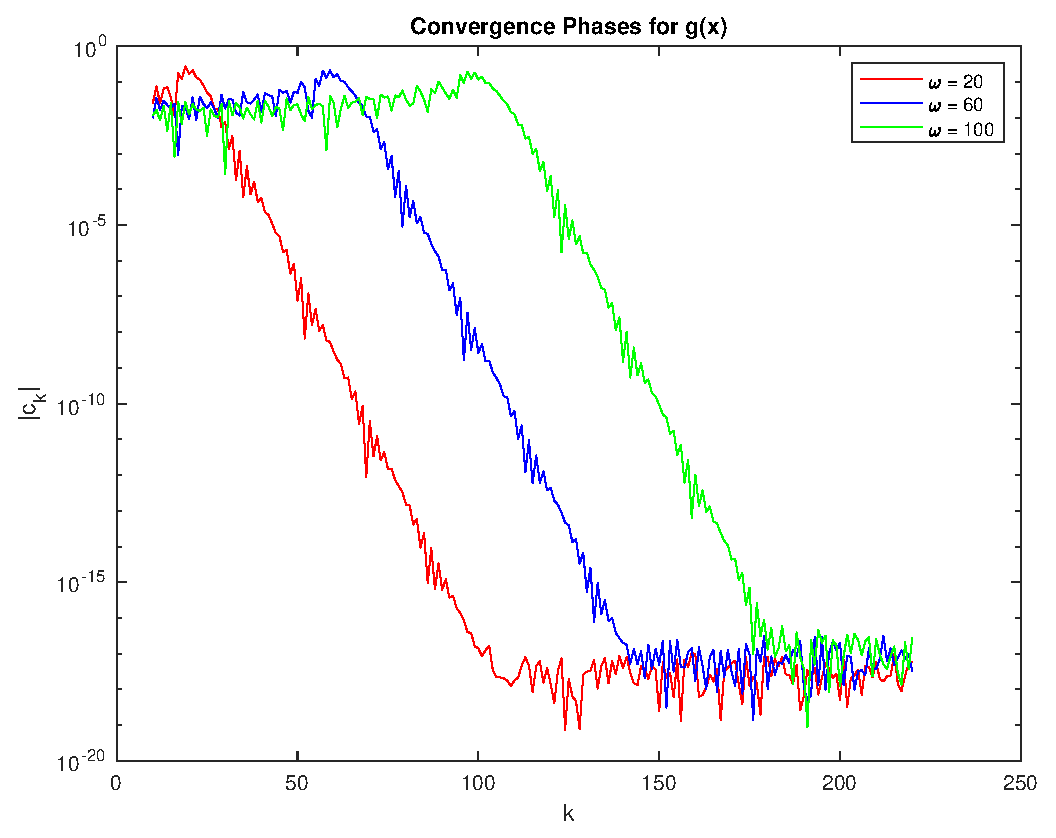
\includegraphics [width=4in]{Lab5_03.eps}
\begin{par}
Since g(x) has a finite radius of convergence and is analytic in the closed Bernstein ellipse, the Chebyshev coefficients for g(x) can be bounded by O(rho\^{}-k) where rho is the radius of the Bernstein ellipse. By solving for the poles, I calculated that rho =\ensuremath{\tilde{\;}} 1.6209. The graph below showcases this bound on the Chebyshev coefficients at the convergence phase can be approximated by 10000 * 1.6209 \^{} -k.
\end{par} \vspace{1em}
\begin{verbatim}
z_0 = ((0.2 + 1i) + sqrt(-4.96 + 0.4 * 1i)) / 2;
z_1 = ((0.2 + 1i) - sqrt(-4.96 + 0.4 * 1i)) / 2;
z_2 = ((0.2 - 1i) + sqrt(-4.96 - 0.4 * 1i)) / 2;
z_3 = ((0.2 - 1i) - sqrt(-4.96 - 0.4 * 1i)) / 2;
rhos = [abs(z_0), abs(z_1), abs(z_2), abs(z_3)];
rho = abs(z_0);
M = 10000;
kstart = 10;
kend = 220;
k = linspace(kstart, kend, kend-kstart+1);
figure5 = figure();
semilogy(k, c_g(k, 2), (20:100), M ./ (rho .^ (20:100)), 'LineWidth', 2);
xlabel('k');
ylabel('|c_k|');
title('Chebyshev Coefficient Bound (M=10000)');
legend('\omega = 20', 'M \rho ^{-k} ');
\end{verbatim}

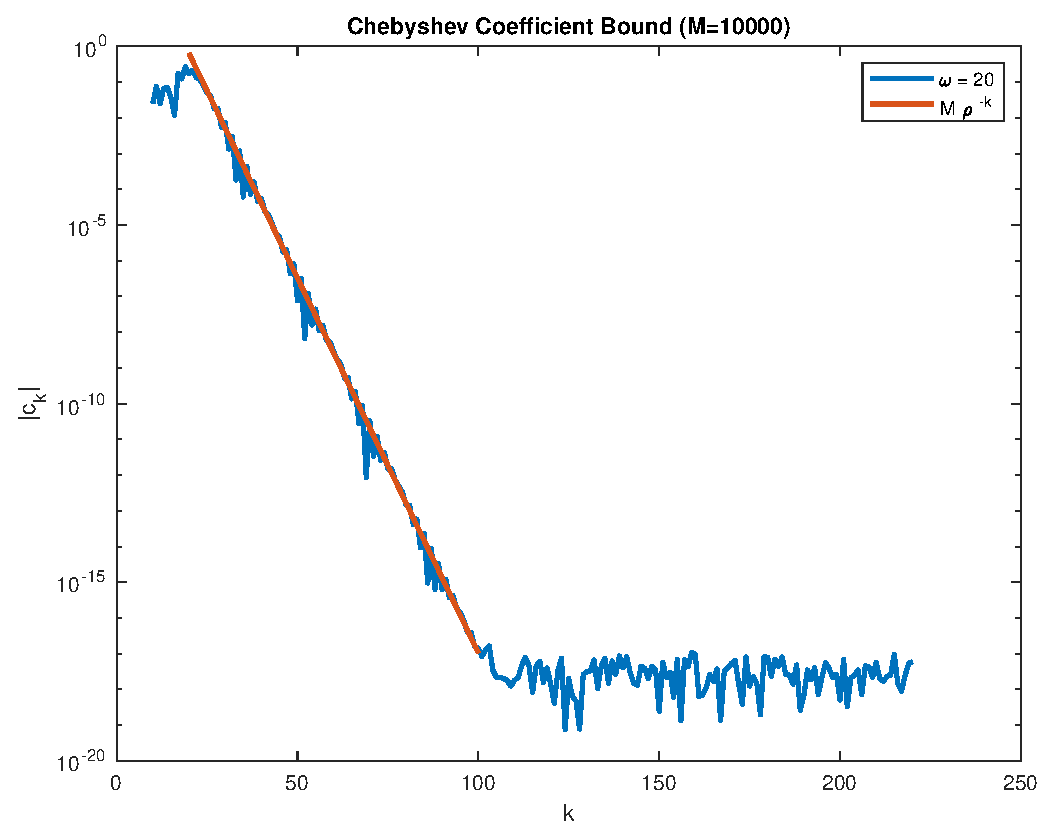
\includegraphics [width=4in]{Lab5_04.eps}


\subsection*{h(x)}

\begin{par}
The graph below plots the Chebyshev coefficients c\_k against k in a semilogy scale. For omega=20, the convergence phase starts from k=10. For omega=60, the convergence phase starts from k=40. For omega=100, the convergence phase starts from k=80. However for all three of these approximations, the convergence is very slow as shown in graph of the left. They all seem to converge somewhere around k=5000.
\end{par} \vspace{1em}
\begin{verbatim}
kstart = 200;
kend = 5000;
k = linspace(kstart, kend, kend-kstart+1);
figure3 = figure();
semilogy(k, c_h(k, 2), '-r', k, c_h(k, 6), '-b', k, c_h(k, 10), '-g');
xlabel('k');
ylabel('|c_k|');
title('Chebyshev Coefficients for h(x) for Large k');
legend('\omega = 20', '\omega = 60', '\omega = 100');

kstart = 10;
kend = 200;
k = linspace(kstart, kend, kend-kstart+1);
figure4 = figure();
semilogy(k, c_h(k, 2), '-r', k, c_h(k, 6), '-b', k, c_h(k, 10), '-g');
xlabel('k');
ylabel('|c_k|');
title('Chebyshev Coefficients for h(x) for small k');
legend('\omega = 20', '\omega = 60', '\omega = 100');
\end{verbatim}

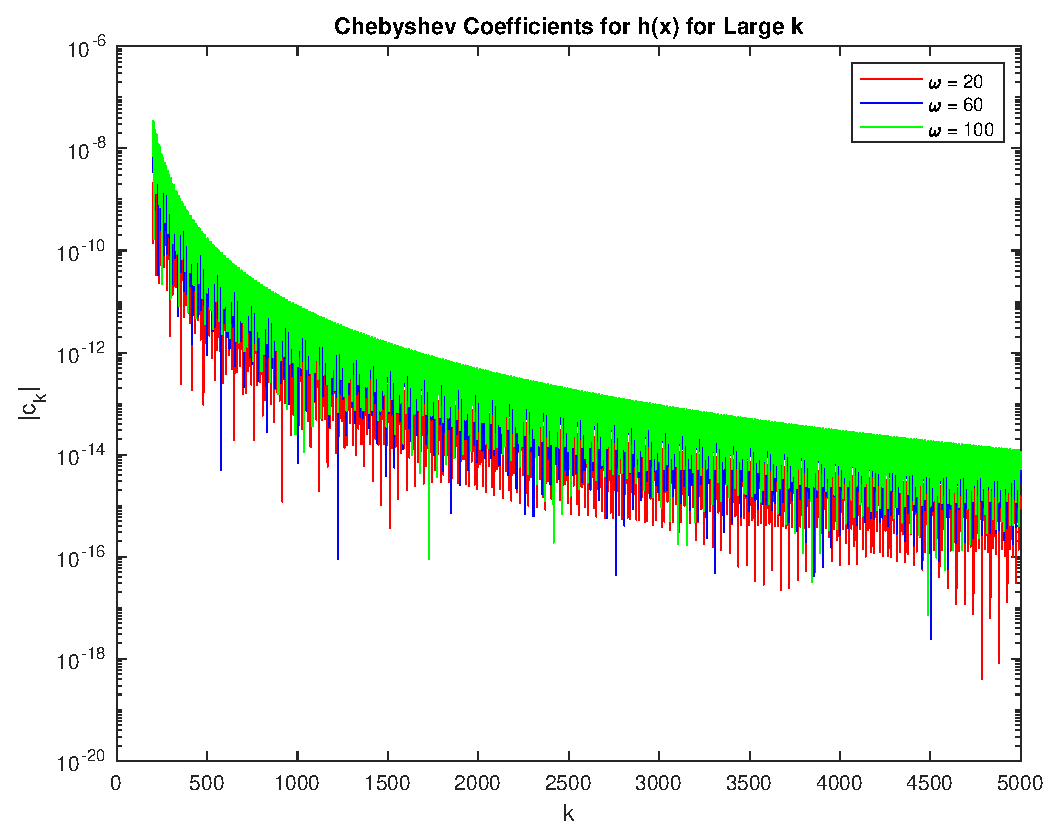
\includegraphics [width=4in]{Lab5_05.eps}

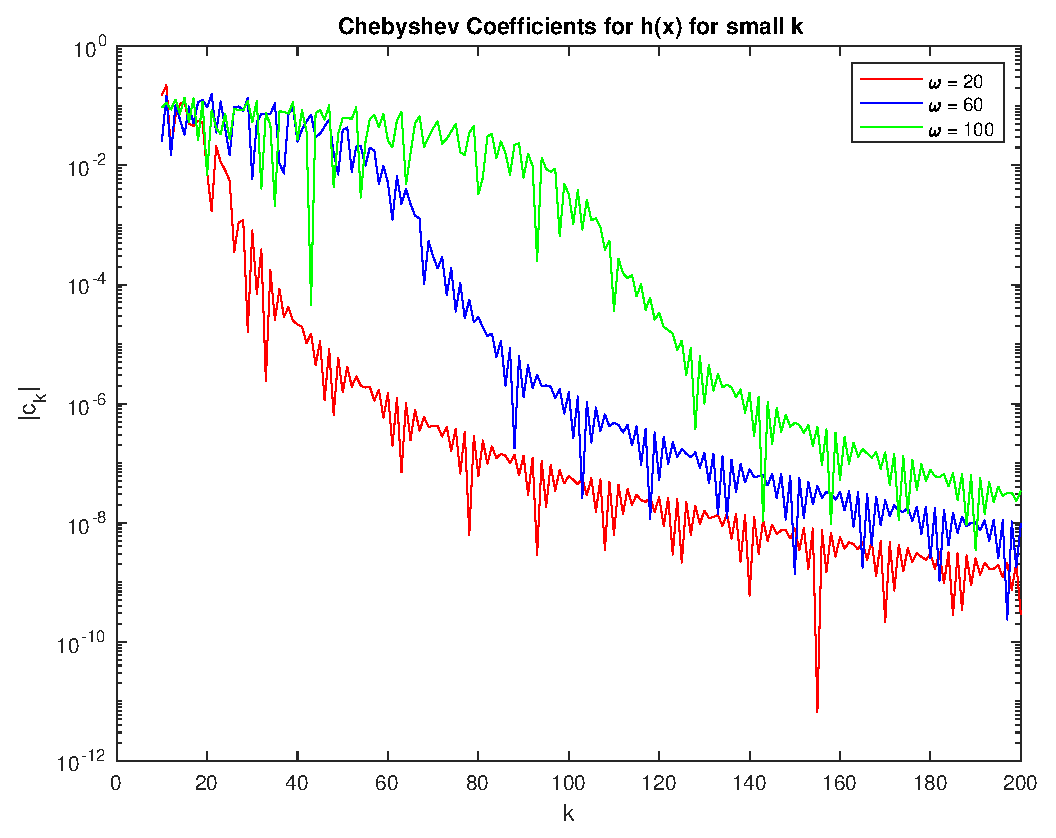
\includegraphics [width=4in]{Lab5_06.eps}
\begin{par}
Since h(x) is twice differentiable and both derivatives are of bounded variation, the Chebyshev coefficients of h(x) can be bounded by O(k\^{}-2). Therefore in the convergence phase, the Chebyshev coefficients c\_k can be approximated by M * k\^{}-2. This is shown in the graph below. However, the bound is not very good. This is likely because the
\end{par} \vspace{1em}
\begin{verbatim}
nu = 2;
M = 0.0000005;
kstart = 20;
kend = 2000;
k = linspace(kstart, kend, kend-kstart+1);
figure6 = figure();
semilogy(k, c_h(k, 2), (20:2000), M ./ ((20:2000) .^ nu), 'LineWidth', 2);
xlabel('k');
ylabel('|c_k|');
title('Chebyshev Coefficient Bound (M=0.0000005)');
legend('\omega = 20', 'M k^{-\nu} ');
\end{verbatim}

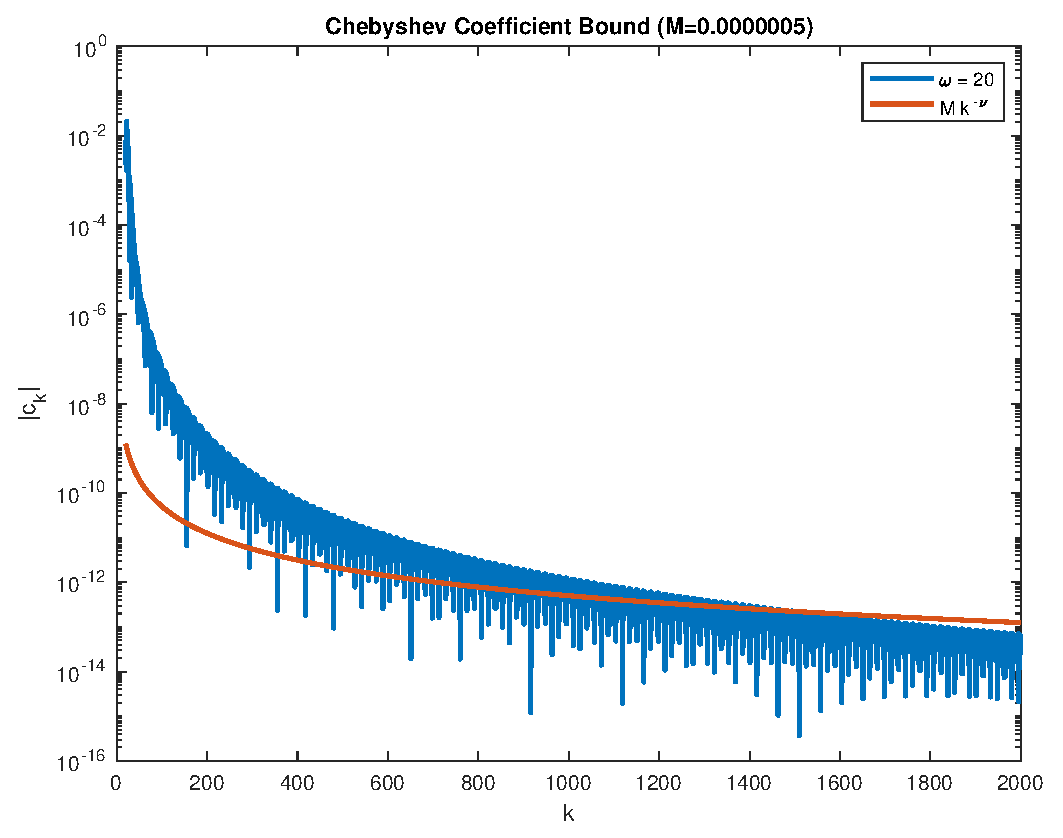
\includegraphics [width=4in]{Lab5_07.eps}
\begin{par}
For the three functions above, the one clear observation is that as omega increases, the convergence phase both starts later and lasts longer. It is also interesting how for all three functions the convergence phases start at almost the same places, with the exception of h(x), whose convergence phase was harder to determine. By looking at all the plots, I can estimate a function to calculate the start of the convergence phase or the length of the preconvergence phase. The estimate I got was that the convergence phases starts at k=0.95*omega.
\end{par} \vspace{1em}



\end{document}

